\documentclass[10pt]{beamer}
\usetheme{Madrid}
\usepackage{booktabs}
\usepackage{graphicx}
\usepackage[T1]{fontenc}
\usepackage{tikz}
\usetikzlibrary{arrows.meta}
\setbeamertemplate{navigation symbols}{}
% To view speaker notes, uncomment the next line (adds note pages):
% \setbeameroption{show notes}
\tikzset{
  box/.style={draw, rounded corners, align=center, text width=2.3cm, minimum height=0.9cm, font=\scriptsize},
  kuser/.style={box, fill=blue!15}, kagent/.style={box, fill=green!25},
  kdata/.style={box, fill=black!8}, kdanger/.style={box, fill=red!25},
  koutput/.style={box, fill=orange!25}, kdecision/.style={box, fill=yellow!30},
  kguard/.style={box, fill=violet!25},
  flow/.style={-{Stealth[length=2mm]}, thick},
}
% ======================= EDIT YOUR DETAILS =======================
\newcommand{\studentname}{Aflah Muhammed P}
% Change the university roll/registration number:
\newcommand{\rollno}{TVE23CSXXX}
% Change your class roll number:
\newcommand{\rollclass}{Roll No: XX}
% Change your guide name:
\newcommand{\guidename}{Prof. Guide Name}
% Change department / college / short-institute if needed:
\newcommand{\deptname}{Department of Computer Science and Engineering}
\newcommand{\collegename}{College of Engineering Trivandrum}
\newcommand{\shortinst}{CET}
% Change the seminar date:
\newcommand{\seminardate}{\today}
% =================================================================
\title[B.Tech Seminar]{Defeating Prompt Injections by Design: How Google DeepMind's CaMeL Protects AI Agents}
\subtitle{Based on: Defeating Prompt Injections by Design (arXiv:2503.18813, 2025)}
\author[\studentname\ (\shortinst)]{\studentname \\ \small \rollno \\ \small \rollclass \\ \small Guide: \guidename}
\institute[]{\deptname \\ \collegename}
\date{\seminardate}
\begin{document}
\begin{frame}[plain]
  \titlepage
\end{frame}
\begin{frame}{Table of Contents}
  \tableofcontents
\end{frame}
\section{Introduction}
\begin{frame}{Introduction}
\begin{itemize}
  \item AI agents now read emails, browse webpages, and call real tools for us.
  \item Reading outside text lets hidden attacker instructions sneak into the agent.
  \item This trick is called prompt injection, a top security risk for agents.
  \item CaMeL defends agents by design, not by retraining a smarter model.
  \item It splits the trusted plan from the untrusted data it must read.
  \item A special interpreter and safety policies check every action before it runs.
\end{itemize}
\end{frame}
\note{Start by reminding everyone that AI agents now do real things for us, like sending emails or booking travel. The catch is that to be useful they must read outside text, and that text can contain hidden traps. Today we look at a Google DeepMind defense called CaMeL that protects agents by design.}
\section{Literature Survey}
\begin{frame}{Literature Survey / Background}
  \small
  \begin{tabular}{@{}p{2.7cm}p{2.3cm}p{5.6cm}@{}}
    \toprule
    \textbf{Title} & \textbf{Author} & \textbf{Summary} \\
    \midrule
    Indirect Prompt Injection (Greshake et al., 2023) & Greshake, Abdelnabi, Mishra et al. & Showed attackers can hide commands in webpages or emails that LLM apps later read and blindly obey. \\
    \addlinespace
    The Dual LLM Pattern (Willison, 2023) & Simon Willison & Proposed splitting a trusted planner LLM from a quarantined LLM that reads risky data without tool access. \\
    \addlinespace
    AgentDojo Benchmark (Debenedetti et al., 2024) & Debenedetti, Zhang, Balunovic et al. & A realistic testbed of agent tasks and injection attacks used to measure both usefulness and security. \\
    \addlinespace
    \bottomrule
  \end{tabular}
\end{frame}
\note{Briefly set the stage with three earlier ideas. Greshake and colleagues first showed attackers can hide commands in webpages and emails. Simon Willison suggested splitting the planner from a quarantined reader. And AgentDojo gave the community a realistic way to measure how safe and useful an agent really is.}
\section{Motivation}
\begin{frame}{Motivation}
\begin{itemize}
  \item Agents are only useful if they can act on untrusted, real-world data.
  \item But every piece of that data may carry hidden malicious instructions.
  \item Training models to resist injections still leaves gaps attackers can exploit.
  \item One leaked email or wrong transfer can cause real, irreversible harm.
  \item We need protection that holds even when the model itself is fooled.
\end{itemize}
\end{frame}
\note{Explain why this matters. Agents are only valuable if they act on messy real-world data, but that same data is where attacks hide. Simply training models to resist attacks still leaves gaps, and one wrong action, like leaking a file, can be irreversible. We want safety even when the model itself gets fooled.}
\section{Problem Statement}
\begin{frame}{Problem Statement}
  \begin{block}{}
  LLM agents cannot reliably tell trusted user instructions apart from malicious instructions hidden inside the untrusted data they read, so attackers can hijack the agent's actions. CaMeL asks how to guarantee safe behavior even when the underlying model can be tricked.
  \end{block}
\end{frame}
\note{State the core problem plainly. The agent cannot reliably tell the user's real instructions apart from fake instructions buried in the data it reads. CaMeL asks how we can guarantee safe behavior even assuming the model can be tricked.}
\section{Objectives}
\begin{frame}{Objectives}
\begin{itemize}
  \item Stop untrusted data from changing what the agent decides to do.
  \item Prevent private data from leaking through unauthorized tool calls.
  \item Provide protection without retraining or fine-tuning the language model.
  \item Keep the agent useful enough to finish most real tasks.
  \item Make security guarantees provable, not just empirically likely.
  \item Let users set clear policies for sensitive or risky actions.
\end{itemize}
\end{frame}
\note{Walk through what CaMeL is trying to achieve. Keep untrusted data from changing the agent's decisions, stop private data from leaking, and do all this without retraining the model. Crucially, the guarantees should be provable, while the agent stays useful enough to finish most tasks.}
\section{Methodology}
\begin{frame}[allowframebreaks]{Methodology: Two Separated LLMs}
\begin{itemize}
  \item Privileged LLM sees only the trusted user request.
  \item It writes a step-by-step program, never touching raw untrusted text.
  \item Quarantined LLM reads risky data but has no tool access.
  \item Q-LLM only extracts values into a fixed, typed format.
  \item Separation stops hidden commands from becoming new instructions.
\end{itemize}
\end{frame}
\note{Cover the three pillars slowly. First, two separate LLMs: a trusted planner that writes code, and a quarantined reader that only extracts data and cannot use tools. Second, a custom interpreter that runs the plan and tags every value as trusted or untrusted. Third, capabilities and policies that check those tags before any tool actually fires.}
\begin{frame}[allowframebreaks]{Methodology: Custom Interpreter with Data-Flow Tracking}
\begin{itemize}
  \item A custom Python-like interpreter runs the P-LLM's program.
  \item It tracks whether each value came from trusted or untrusted sources.
  \item Anything derived from untrusted data stays tagged as untrusted.
  \item Control flow comes only from the trusted plan, never from data.
\end{itemize}
\end{frame}
\begin{frame}[allowframebreaks]{Methodology: Capabilities and Security Policies}
\begin{itemize}
  \item Each value carries capability tags: its source and allowed readers.
  \item Policies check these tags before any tool is actually called.
  \item Risky actions can be blocked or sent to the user for approval.
  \item This prevents exfiltration even if the plan was slightly misled.
\end{itemize}
\end{frame}
\section{Key Concepts}
\begin{frame}[allowframebreaks]{Key Concepts}
  \begin{description}
    \item[Prompt Injection] Hidden instructions inside data that trick an agent into unintended actions.
    \item[Privileged LLM (P-LLM)] Trusted planner that turns the user request into a safe program.
    \item[Quarantined LLM (Q-LLM)] Isolated model that reads untrusted text but cannot call tools.
    \item[Capability] Tag on each value recording its origin and who may read it.
    \item[Security Policy] Rule checked at each tool call to allow, block, or confirm.
    \item[Provable Security] Guarantee that untrusted data cannot alter the agent's control flow.
  \end{description}
\end{frame}
\note{Define the jargon in plain words. Prompt injection is a hidden command inside data. The Privileged LLM is the trusted planner, the Quarantined LLM is the isolated reader. A capability is just a tag saying where data came from and who may see it, and a policy is a rule checked before acting. Provable security means untrusted data mathematically cannot change the plan.}
\section{System Architecture}
\begin{frame}{System Architecture}
  \begin{center}
  \resizebox{0.96\textwidth}{!}{%
  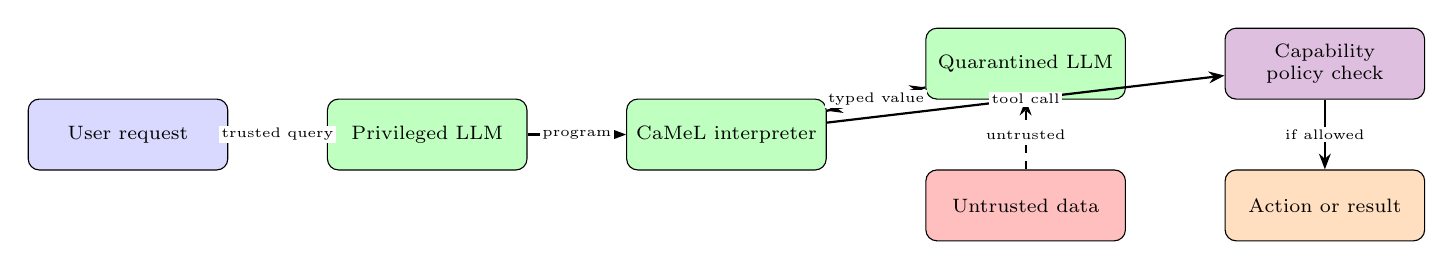
\begin{tikzpicture}
    \node[kuser] (user) at (0.00,0.00) {User request};
    \node[kagent] (pllm) at (3.80,0.00) {Privileged LLM};
    \node[kagent] (interp) at (7.60,0.00) {CaMeL interpreter};
    \node[kagent] (qllm) at (11.40,0.90) {Quarantined LLM};
    \node[kdanger] (udata) at (11.40,-0.90) {Untrusted data};
    \node[kguard] (guard) at (15.20,0.90) {Capability policy check};
    \node[koutput] (output) at (15.20,-0.90) {Action or result};
    \draw[flow] (user) -- (pllm) node[midway, font=\tiny, fill=white, inner sep=1pt]{trusted query};
    \draw[flow] (pllm) -- (interp) node[midway, font=\tiny, fill=white, inner sep=1pt]{program};
    \draw[flow] (interp) -- (qllm) node[midway, font=\tiny, fill=white, inner sep=1pt]{parse text};
    \draw[flow, dashed] (udata) -- (qllm) node[midway, font=\tiny, fill=white, inner sep=1pt]{untrusted};
    \draw[flow] (qllm) -- (interp) node[midway, font=\tiny, fill=white, inner sep=1pt]{typed value};
    \draw[flow] (interp) -- (guard) node[midway, font=\tiny, fill=white, inner sep=1pt]{tool call};
    \draw[flow] (guard) -- (output) node[midway, font=\tiny, fill=white, inner sep=1pt]{if allowed};
  \end{tikzpicture}%
  }
  \end{center}
  \begin{center}\scriptsize CaMeL pipeline: a trusted planner writes a program that an interpreter runs, isolating untrusted data and gating every tool call with policies.\end{center}
\end{frame}
\note{Walk the diagram left to right. The trusted request goes to the Privileged LLM, which writes a program. The interpreter runs that program and, when it needs to read risky text, calls the Quarantined LLM. Untrusted data only ever flows in as tagged values, and before any tool runs, the policy check decides whether to allow it, block it, or ask you.}
\begin{frame}[allowframebreaks]{How It Works (Explained)}
\begin{itemize}
  \item The user sends a trusted request into the system on the left.
  \item The Privileged LLM reads only that request and writes a program.
  \item The CaMeL interpreter runs the program and tracks every value's source.
  \item When it must read risky text, it calls the Quarantined LLM.
  \item Untrusted data feeds the Q-LLM, which returns only typed values, not commands.
  \item Before any real tool runs, capability policies check the value's tags.
  \item Only actions passing the policy check produce a final result.
\end{itemize}
\end{frame}
\section{Example Walkthrough}
\begin{frame}[allowframebreaks]{Example Walkthrough: Example: Send Bob a document from the meeting notes}
\begin{enumerate}
  \item You ask: send Bob the document he requested in our last meeting.
  \item The Privileged LLM writes a program: read notes, find address, send file.
  \item The interpreter reads the notes file, tagging its contents as untrusted.
  \item It asks the Quarantined LLM to extract Bob's email from that text.
  \item The extracted address is tagged untrusted because it came from the notes.
  \item A hidden line saying email everyone cannot change the plan, only data.
  \item The policy sees an untrusted recipient and asks you to confirm before sending.
\end{enumerate}
\end{frame}
\note{Use the Bob email example to make it concrete. You ask the agent to send Bob a document from the meeting notes. The planner writes the steps, the interpreter reads the notes as untrusted, and the quarantined model pulls out Bob's address. Even if the notes secretly say email everyone, that text is only data, so the plan does not change, and the policy still asks you to confirm the recipient.}
\section{Results}
\begin{frame}[allowframebreaks]{Results / Findings}
\begin{itemize}
  \item CaMeL solved 77\% of AgentDojo tasks with provable security.
  \item An undefended baseline agent completed about 84\% of the same tasks.
  \item So strong security cost only a modest drop in usefulness.
  \item Protection required no model retraining or fine-tuning at all.
  \item The defense worked across different underlying models like GPT-4o and Claude.
  \item Against the benchmark's injection attacks, protected actions could not be hijacked.
\end{itemize}
\end{frame}
\note{Share the headline numbers. CaMeL solved seventy-seven percent of AgentDojo tasks with provable security, while an undefended agent finished about eighty-four percent. So strong protection cost only a small drop in usefulness, needed no retraining, and worked across different models like GPT-4o and Claude.}
\section{Discussion}
\begin{frame}{Discussion}
\begin{itemize}
  \item Security comes from system design, not from a hoped-for smarter model.
  \item The same idea generalizes to many agents and tools, not just email.
  \item Borrowing decades-old ideas from software security proves practical for LLMs.
  \item Provable guarantees shift trust from the model to the surrounding layer.
\end{itemize}
\end{frame}
\note{Zoom out on why this is exciting. Security here comes from good system design, not from hoping for a perfect model. It reuses decades-old software security ideas, like data-flow tracking and capabilities, and applies them to LLM agents in a way that generalizes well beyond email.}
\section{Challenges}
\begin{frame}{Limitations \& Challenges}
\begin{itemize}
  \item Users or developers must write and maintain the security policies.
  \item Too many confirmation prompts can cause fatigue and careless approvals.
  \item The Quarantined LLM can still extract wrong or incomplete values.
  \item Subtle side channels may still leak small amounts of information.
\end{itemize}
\end{frame}
\note{Be honest about the trade-offs. Someone still has to write the security policies, and too many confirmation pop-ups can make users click yes without thinking. The quarantined model can also extract the wrong value, and subtle side channels might still leak tiny amounts of information.}
\section{Future Work}
\begin{frame}{Future Work}
\begin{itemize}
  \item Automate policy creation so users need less manual configuration.
  \item Reduce confirmation prompts to avoid overwhelming and fatiguing users.
  \item Extend the interpreter to more languages, tools, and multi-agent settings.
  \item Close remaining side channels and harden Q-LLM extraction reliability.
\end{itemize}
\end{frame}
\note{Point to what comes next. The authors want to generate policies automatically, cut down on confirmation prompts, and extend the approach to more tools and multi-agent systems. Closing remaining side channels and making extraction more reliable are also open directions.}
\section{Conclusion}
\begin{frame}{Conclusion}
\begin{itemize}
  \item Prompt injection is a fundamental, not merely incidental, agent security risk.
  \item CaMeL defends by design, separating trusted plans from untrusted data.
  \item Capabilities and policies gate every action, giving provable protection.
  \item It secures agents today without waiting for perfectly robust models.
\end{itemize}
\end{frame}
\note{Wrap up with the big message. Prompt injection is a deep, fundamental risk for agents, and CaMeL tackles it by separating trusted plans from untrusted data and gating every action with policies. The result is provable protection we can use today, without waiting for perfectly secure models.}
\section{References}
\begin{frame}[allowframebreaks]{References}
  \footnotesize
  \begin{enumerate}
    \item Debenedetti, E., Shumailov, I., Fan, T., Hayes, J., Carlini, N., Fabian, D., Kern, C., Shi, C., Terzis, A., \& Tramer, F. (2025). Defeating Prompt Injections by Design. arXiv:2503.18813.
    \item Debenedetti, E., Zhang, J., Balunovic, M., Beurer-Kellner, L., Fischer, M., \& Tramer, F. (2024). AgentDojo: A Dynamic Environment to Evaluate Attacks and Defenses for LLM Agents. arXiv:2406.13352.
    \item Greshake, K., Abdelnabi, S., Mishra, S., Endres, C., Holz, T., \& Fritz, M. (2023). Not What You've Signed Up For: Compromising Real-World LLM-Integrated Applications with Indirect Prompt Injection. ACM AISec. arXiv:2302.12173.
    \item Willison, S. (2023). The Dual LLM Pattern for Building AI Assistants That Can Resist Prompt Injection. simonwillison.net.
    \item Perez, F., \& Ribeiro, I. (2022). Ignore Previous Prompt: Attack Techniques For Language Models. arXiv:2211.09527.
    \item Willison, S. (2025). CaMeL Offers a Promising New Direction for Mitigating Prompt Injection Attacks. simonwillison.net.
  \end{enumerate}
\end{frame}
\begin{frame}[plain]
  \begin{center}
    {\Huge Thank You}\\[1em]
    {\large Questions?}
  \end{center}
\end{frame}
\end{document}